%!TEX root = ../Principal.tex
%Capa do Trabalho
\imprimircapa

%Folha de Rosto
%* indica que tem ficha catalográfica
\imprimirfolhaderosto*

% ---
% Caso a Biblioteca da UDESC forneça, utilize o comando
% ---
% \begin{fichacatalografica}
%     \includepdf{fig_ficha_catalografica.pdf}
% \end{fichacatalografica}

% ---
% Geração da Ficha Catalográfica Via LaTeX
% ---
% \begin{fichacatalografica}
% 	\vspace*{\fill}					% Posição vertical
% 	\begin{center}					% Minipage Centralizado
% 	\begin{minipage}[c]{12.5cm}		% Largura

% 	\imprimirautor

% 	\hspace{0.5cm} \imprimirtitulo  / \imprimirautor. --
% 	\imprimirlocal, \imprimirdata-

% 	\hspace{0.5cm} \pageref{LastPage} p. : il. (algumas color.) ; 30 cm.\\

% 	\hspace{0.5cm} \imprimirorientadorRotulo~\imprimirorientador\\

% 	\hspace{0.5cm}
% 	\parbox[t]{\textwidth}{\imprimirtipotrabalho~--~\imprimirinstituicao,
% 	\imprimirdata.}\\

% 	\hspace{0.5cm}
% 		1. Tópico 01.
% 		2. Tópico 02.
% 		I. Prof. Dr. xxxxx.
% 		II. Universidade do Estado de Santa Catarina.
% 		III. Centro de Ciências Tecnológicas.
% 		IV. identificação xxxx\\

% 	\hspace{8.75cm} CDU 02:121:005.7\\

% 	\end{minipage}
% 	\end{center}
% \end{fichacatalografica}

% % ---
% % Folha de Aprovação
% % ---
% % Exemplo de folha de aprovação antes da Banca. Após isso, incluia o pdf digitalizado com as assinaturas%
% % 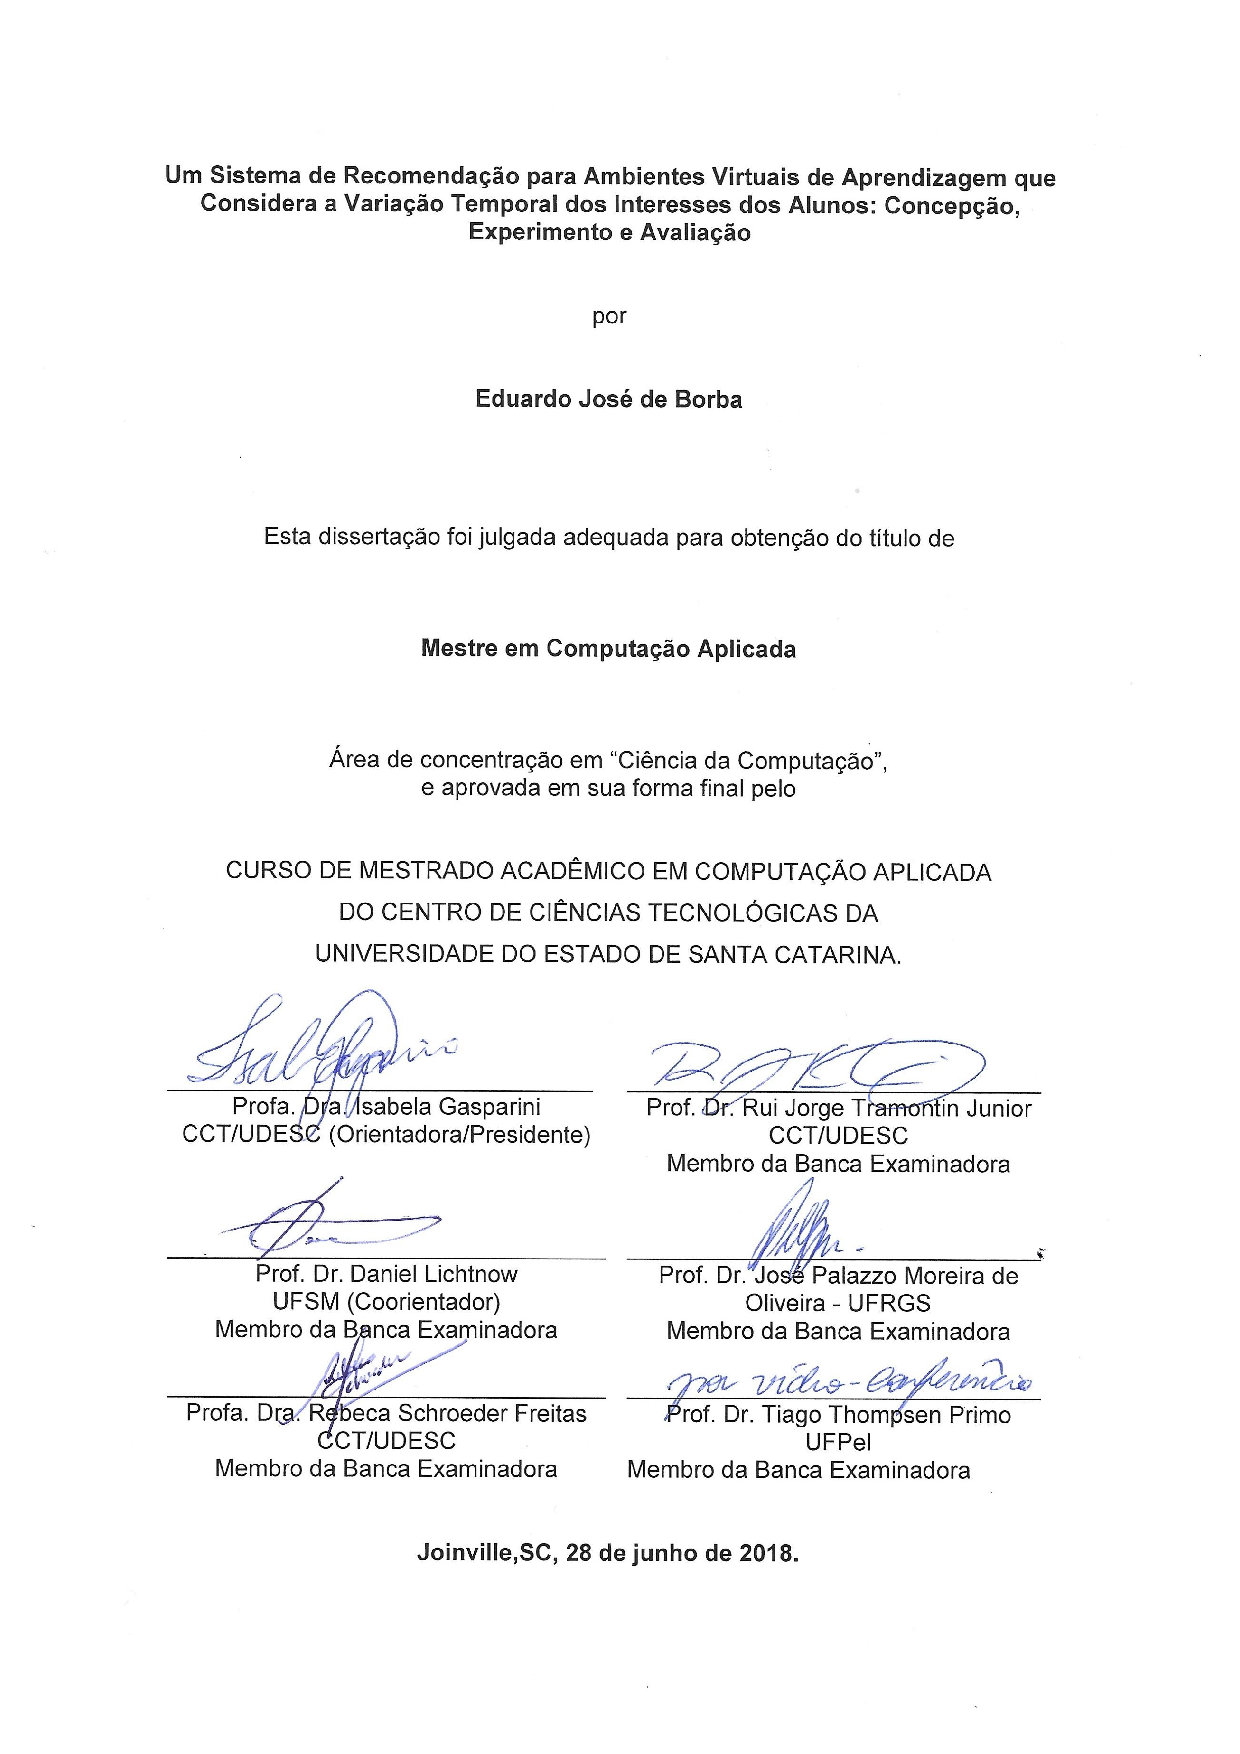
\includepdf{folhadeaprovacao_final.pdf}
\begin{folhadeaprovacao}
	\begin{center}
		{\ABNTEXchapterfont\bfseries\imprimirautor}
		\vspace{2em}

			\ABNTEXchapterfont\bfseries\imprimirtitulo

	\end{center}
		\vspace{1em}
		{\justify
    Dissertação apresentada ao Programa de Pós-Graduação em Computação Aplicada, da Universidade do Estado de Santa
    Catarina, como requisito parcial para a obtenção do grau de Mestre em Computação Aplicada.}
	 \vspace{2em}
	\noindent

	{\justify \bfseries Banca Examinadora}

  \vspace{2em}

  \noindent{Orientadora:\hfill \assinatura*{\textbf{\imprimirorientadorRotulo \imprimirorientador} \\ Universidade do Estado de Santa Catarina (UDESC)}}

  \noindent{Coorientador:\hfill \assinatura*{\textbf{\imprimircoorientadorRotulo \imprimircoorientador} \\ Universidade Federal de Santa Marina (UFSM)}}

  \noindent{Membros:}

	\noindent{\assinatura*{\textbf{Dr. Rui Jorge Tramontin Junior} \\ Universidade do Estado de Santa Catarina (UDESC)}}
  \noindent{\assinatura*{\textbf{Dra. Rebeca Schroeder Freitas} \\ Universidade do Estado de Santa Catarina (UDESC)}}
  \noindent{\assinatura*{\textbf{Dr. Tiago T. Primo} \\ Universidade Federal de Pelotas (UFPel)}}
  \noindent{\assinatura*{\textbf{Dr. José Palazzo M. de Oliveira} \\ Universidade Federal do Rio Grande do Sul (UFRGS)}}

    \vspace*{\fill}
    \begin{center}
    	\imprimirlocal,\,\imprimirfulldata
    \end{center}
\end{folhadeaprovacao}

% ---
% Dedicatória
% ---
% \begin{dedicatoria}
% Dedico este trabalho aos meus familiares, amigos, colegas e professores que me acompanharam e me deram forças nessa magnífica trajetória.
% \end{dedicatoria}

% % ---
% % Agradecimentos
% % ---
% \begin{agradecimentos}
% Gostaria de agradecer...

% Aqui devem ser colocadas os agradecimentos às pessoas que de alguma forma contribuíram para a realização do trabalho.
% \end{agradecimentos}

% ---
% Epígrafe
% ---
% \begin{epigrafe}
% ``Independentemente das circunstâncias, devemos ser sempre humildes, recatados e despidos de orgulho.''
% \\
% \par
% Dalai Lama
% \end{epigrafe}

% ---
% RESUMOS
% ---

% Português
\begin{resumo}
  Sistemas de Recomendação (SR) são ferramentas de \textit{software} que sugerem itens para os usuários de forma automatizada e
  personalizada, sem a necessidade do usuário formular uma consulta para encontrar os itens do seu interesse. Esses
  sistemas são explorados em Ambientes Virtuais de Aprendizagem (AVA) com o objetivo de reduzir alguns problemas
  existentes nesses ambientes quando a quantidade de materiais disponíveis é grande, tais como: sobrecarga cognitiva,
  dificuldade de encontrar os materiais do seu interesse e muitos materiais nunca serem utilizados. Pesquisadores da
  área argumentam que os algoritmos de SRs tradicionais não são suficientes para os AVAs, sendo necessário um nível
  maior de personalização da situação do usuário, como considerar informações do seu contexto. O objetivo desse trabalho é
  avaliar se a aplicação do decaimento dos interesses do usuário em itens acessados anteriormente em SRs voltados a AVAs
  influencia o desempenho da abordagem de recomendação e a percepção dos alunos sobre as recomendações recebidas. O
  algoritmo com decaimento proposto combina a (1) similaridade do perfil do usuário
  (representado pelos materiais acessados pelo usuário) com os itens disponíveis para a recomendação com a (2) recência
  do acesso ou uso desse materiais, além da (3) informação se aquele item disponível para a recomendação já foi acessado
  ou não. A proposta leva em conta que o ritmo de estudo dos alunos pode ser diferente, portanto a recência é
  considerada em relação à sequência de itens acessados e não ao tempo absoluto (em segundos) desde o acesso. A proposta
  desse trabalho foi incorporada ao ambiente \adaptwebspace e avaliada através de um experimento utilizando um Minicurso
  de Algoritmos e Linguagem de Programação ministrado no ambiente. O algoritmo proposto foi comparado à abordagem
  Baseada em Conteúdo Tradicional utilizando uma estratégia \textit{Between Subjects}. Os resultados mostraram
  que existe diferença significativa na Cobertura, F-measure e em uma das questões do sobre a percepção do usuário e que
  a abordagem com Decaimento teve resultados melhores nessas métricas. Portanto, as  duas hipóteses alternativas
  definidas para o experimento foram aceitas e indicam que considerar o Decaimento em um SR
  para AVAs influencia positivamente o desempenho do algoritmo e a percepção dos alunos sobre as recomendações.

  \vspace{\onelineskip}

  \noindent
  \textbf{Palavras-chaves}: Sistema de Recomendação; Sensível ao Tempo; Sensível ao Contexto; Decaimento; Ambiente Virtual de Aprendizagem; \adaptweb.
\end{resumo}

% Inglês
\begin{resumo}[Abstract]
 \begin{otherlanguage*}{english}
  	Recommender Systems (RS) are software tools that provide items as suggestions to users automatically and personalized to his
    interests, without the need to formulate a search argument to achieve this. This systems are applied to Virtual Learning
    Environments (VLE) aiming to reduce some drawbacks existing in these enviroments when the number of available items is
    huge, e.g., cognitive overload, difficulty finding items of user's interest or some materials never get accessed. Researchers
    in this area argues that traditional RS approaches are not enough for VLE, being required a major level of personalization
    to user's current context. This work goals is evaluate whether the use of Decay on user's interest for past items
    on RS for VLEs influence the algorithm performance and the user's perception of the recommendations. The proposed
    algorithm combines (1) similarity between user profile (represented by the materials accessed by the user) with the items
    available to recommendation with (2) the recency of materials accessed by the user and (3) the information about if
    the item available to be recommended was accessed or not. The proposal takes into account that each learner can have
    a different study rhythm, therefore the recency considers the sequence of items accessed and not the absolute time (in
    seconds) from the access. The proposal of this work was incorporated to the \adaptwebspace environment and evaluated
    through an experiment using an Algorithms and Programming Language's course. The proposal was compared to the Content-Based traditional approach
    through using a Between Subjects strategy. The results show that there is significant difference on the Coverage,
    F-measure and in one of the questions about the user's perception and that the approach with Decay had better results
    in these metrics. Therefore, both alternative hypothesis defined for the experiment were accepted and it indicates
    that consider the Decay on a RS for VLEs influences the algorithm performance and the user's perception of the recommendations.
    \vspace{\onelineskip}

    \noindent
    \textbf{Keywords}: Recommender System; Time-Aware; Context-Aware; Decay; Virtual Learning Environment; \adaptweb.
 \end{otherlanguage*}
\end{resumo}

% ---
% Lista de Figuras
% ---
\pdfbookmark[0]{\listfigurename}{lof}
\listoffigures*
\cleardoublepage
% ---

% ---
% Lista de Tabelas
% ---
\pdfbookmark[0]{\listtablename}{lot}
\listoftables*
\cleardoublepage